\documentclass{article}
\input /Users/vigon/visible/MesRacoursis2015

\def\dessin{\ \linebreak \vspace{0.5cm}  \linebreak  DESSIN  \vspace{1cm} \ \linebreak   }



\def\loi{\text{loi}}
\def\std{\text{std}}

\def\mean{\mathrm{mean}}
\title{Stat's trick}



\begin{document}


\maketitle



\section{Introduction : c'est quoi les stats ? }


   
Soit $x=[x_0,...,x_{p-1}]\in \mathbb R^p$. Nous notons :
 \begin{alignat*}{1}
 \mean(x) &= \frac 1 p   \sum_i x_i \\
 \std^2(x) &= \frac 1 {p-1} \sum_i \Big(x_i - \mean(x) \Big)^2\\
  \std (x) &= \sqrt{\std^2(x)}
  \end{alignat*}
   Ces notations sont inspirées de numpy. Mais attention, pour calculer $\std(x)$  il faut faire   \verb$np.std(X,ddof=1)$  (pour le $\frac1{p-1}$ devant la somme). 
   
 
  \begin{exo}
   Vérifiez que pour $a,b\in \mathbb R$, $\mean(ax+b) = a \, \mean(x) + b$ et $\std^2(ax+b)=a^2 \, \std(x)$.
  \end{exo}


Considérons maintenant une va $X_0$ d'espérance $\mu$ et de variance $\sigma^2$.   

Les statisitques commencent quand on se demande comment on peut estimer  $\mu,\sigma^2$ à partir d'observations $X=[X_0,...,X_{p-1}]$ (qui sont toutes des copies indépendantes de notre va initiale).  Le premier élément de réponse c'est que : 
\begin{alignat}{1}
\mu &  \simeq \mean(X) \\
\sigma^2  & \simeq \std^2(X)
\end{alignat}

Mais quelle est la qualité de ces estimations ?  Plus précisémment : 
\begin{itemize}
\item Quel est l'éloignement entre $\mu$   et $\mean(X) $ ?    réponse:   LFGN, TCL
\item Quelle sera la loi de $ \mean(X)$ et $\std^2(X)$ ?  réponse:  théorème de Cochrane.
\item Puis-je donner un intervalle très probable pour $\mu$ ? réponse: intervalle de confiance. 
\item Puis-je affirmer que $\mu=0$ lorsque que $\mean(X)=0.0034123$ ? réponse: test statistique. 
\end{itemize}
Nous répondrons à ces questions dans ce document. Mais attention, il s'agit d'une initiation très sommaire aux statistiques ; en espérant que cela vous donne des jalons  qui vous aideront si vous deviez faire des statistiques plus poussées.  


\begin{exo} Pourquoi a-t-on mis $\frac 1 {p-1}$ et pas $\frac 1 p $ dans l'expression de $\std^2$ ?    
\end{exo}








 



\section{Convergence en loi}


\subsection{Informatiquement}

La convergence ps (presque sûre) c'est la convergence 'habituelle' :     Supposons que $X_n$ sont des réels aléatoires,   $X_n   \xrightarrow{\text{ps}} X_\infty$ signifie que les nombres $X_n$ convergent vers le nombre $X_\infty$.   Pour illustrer une convergence p.s. il suffit de tracer: 
$$
\mathrm{plot}( [0,1,...,], [X_0,X_1,...])   
$$
 On verra une courbe qui se rapproche de la valeur $X_\infty$.  On peut éventuellement relancer plusieurs fois le programme (ou bien superposer plusieurs simulations) pour vérifier que cette convergence à lieu à chaque fois (=presque surement). 


La convergence en loi c'est la convergence des "histogrammes". Pour l'illustrer on est obligé de considérer plusieurs copies indépendantes  $(X^i_n,X^i_\infty)_i$ de $(X_n,X_\infty)$.  On peut choisir $n$ grand (ex $n=100$)    et tracer les histogrammes:
\begin{alignat}{1}
&\mathrm{hist}(  [X^0_{100}, X^1_{100},X^2_{100},...]) \\
&\mathrm{hist}(  [X^0_{\infty}, X^1_{\infty},X^2_{\infty},...])
\end{alignat}
Ces histogrammes devraient se superposer (si $n$ est assez grand, si le nombre de simulation est assez grand par rapport au nombre de batons).

Cependant, en pratique, on dit plutot que $X_n$ converge en loi vers un loi donnée (ex : exponentielle). Dans ce cas, il faut superposer le premier histogramme avec la densité de la loi exponentielle : 
\begin{alignat}{1}
&\mathrm{hist}(  [X^0_{100}, X^1_{100},X^2_{100},...]) \\
x&=\mathrm{linspace(...)}\\
&\mathrm{plot}(  x,  \mathrm{exp}(-x) ])
\end{alignat}

\subsection{Définition}

Fixons nous  $E$ un espace. Typiquement $E=\mathbb R$ ou $E=\mathbb R^p$ ou encore $E$ est un espace de trajectoires (=fonctions de $\mathbb R_+$ dans $\mathbb R^n$). 

Un ensemble de fonctions tests sur $E$ est un ensemble $\Phi$ de fonctions qui caractérise la loi des objets aléatoires à valeurs dans $E$ : 
$$
\fo \ph \in \Phi :   \mathbf E[ \ph(X_1)]=\mathbf E[\ph(X_2) ]   \qq \equi \qq \Pr[X_1\in dx] = \Pr[X_2\in dx]  
$$


L'ensemble des fonctions continues bornée $\bo C_b(E)$ est un ensemble de fonctions testes très important, car il est utilisé pour définir la convergence en loi : 
$$
X_n   \xrightarrow{\text{loi}}   X   \qq \equi \qq     \fo \ph \in  \bo C_b(E) \      \mathbf E[ \ph(X_n)] \to \mathbf E[\ph(X)]
$$

Attention :  la convergence en loi n'est pas vraiment une convergence entre des objets aléatoires, mais bien une convergence entre leurs lois. Parfois, il vaut mieux noter : 
$$
\text{loi} (X_n) \to \loi(X)
$$
On peut aussi utiliser des notations mixtes, ex  : 
 $$
 X_n   \xrightarrow{\text{loi}}   \bo N(0,1)
 $$

\subsection{Exemple à avoir en tête}

\begin{itemize}

\item Si $\text{loi}(X_n) = \de_{x_n}$ et si $x_n \to x$
$$
X_n   \xrightarrow{\text{loi}}     
$$
Exo : vérifiez-le avec la définition. Vérifiez aussi que ça ne marcherait pas si on avait choisi comme ensemble de fonction tests, les indicatrices par exemple. 

\item Le point précédent peut se déduire de l'implication générale suivante:
$$
X_n   \xrightarrow{\text{ps}}  X  \qq \imp \qq       X_n   \xrightarrow{\text{loi}}  X
$$
L'implication inverse est complètement fausse: considérons des va $(X_n),X$  indépendantes, non constantes,  de même loi.  On a  $ X_n   \xrightarrow{\text{loi}}  X$ (rappelez vous que cela signifie $\loi(X_n) \to \loi(X)$).  Pourtant, du fait de l'indépendances, la suite $n\to X_n$ ne se stabilise jamais, donc, pas de convergence ps.  
\item Cependant il y a un cas où l'on a une l'implication dans l'autre sens: Soit $c$ une constante
$$
X_n   \xrightarrow{\text{loi}}  c  \qq \imp X_n   \xrightarrow{\text{ps}}  c
$$ 
 Pour comprendre cela, pensez aux histogrammes : la convergence en loi vers une constante, implique que toutes les trajectoires finissent nécessairement dans le baton qui contient $c$. C'est   bien une convergence ps.   {\tiny ( techniquement, il s'agit d'une convergence en proba, mais c'est quasi pareil)}
 \item Si $f$ est une fonction continue on a
$$
X_n  \xrightarrow{\text{loi}}  X \text{ et }  Y_n \xrightarrow{\text{ps}}  Y   \qq \mathrm{ alors } \qq  f(X_n,Y_n) \xrightarrow{\text{loi}} f(X,Y)
$$
Cette implication est fausse quand on considère deux converges en loi. Prenons par exemple la fonction continue $f(x,y) = x+y$.  Prenons $Z$ et $Z'$ deux va indépendantes non constante et de même loi. Posons $\fo X_n = Z$ et $\fo n  Y_n = - Z $.  On a : $X_n \xrightarrow{\text{loi}} Z$ et  $Y_n \xrightarrow{\text{loi}} Z'$. Pourtant ...  

\item Si $\loi(X_n) = \frac 1n \de_0 +  \frac  {n-1}{n} \de_{1-\frac 1 n}$ alors
$$
X_n  \xrightarrow{\text{loi}}
$$
\end{itemize}

\subsection{Caractérisation}


\begin{itemize}
\item Dans le cas $E=\mathbb R$.  Rappelons que la fonction caractérisitique d'une va $X$ c'est $\text{Carac}_X(u)=\mathbf E[e^{iuX}]$.   On a :
$$
X_n   \xrightarrow{\text{loi}}   X   \qq \equi \qq      \fo u \   \text{Carac}_{X_n} (u)  \xrightarrow[n\to \infty]{}   \text{Carac}_X(u)
$$
Remarque : Cela revient à dire que l'ensemble des fonctions tests  $\{e^{iu\cdot} : u\in \mathbb R \}$  est tout aussi bon que  $\bo C_b(\mathbb R)$ pour définir la convergence en loi.

\item  La convergence en loi de $X_n$ vers $X$ équivaut au fait que, pour tout $a,b$ telle que $ \Pr[X=a]=\Pr[X=b]=0$ on a : 
$$
\Pr\Big[X_n\in ]a,b[  \Big] \to \Pr\Big[X\in ]a,b[  \Big]
$$
La condition $ \Pr[X=a]=\Pr[X=b]=0$ est importante. Exo :  Trouvez un exemple très très simple où $X_n\to X$ en loi, et tel que 
$$
\Pr\Big[X_n\in ]0,1[  \Big] \to  1  \qq \mathrm{ mais } \qq \Pr\Big[X\in ]0,1[  \Big] = 0
$$
\end{itemize}











\section{Théorème central limite}



\subsection{Enoncé}


Soit $X=[X_0,X_1,...]$ une suite de va iid d'espérance $\mu$ et de variance $\sigma^2<\infty$. Notons  $X_{:n}=[X_0,...,X_{n-1}]$.   

\begin{theorem}
La version centrée-réduite de $\mathrm{sum} (X_{:n})$ converge en loi vers une $\bo N(0,1)$. 
\end{theorem}

Précisons : l'espérance et la variance de $\mathrm{sum} (X_{:n})$ valent respectivement $n\mu$ et $n \sigma^2$, ainsi :
$$
\frac {\mathrm{sum}(X_{:n}) - n \mu}{\sigma \sqrt{n} }   \xrightarrow[n\to \infty]{\text{loi}} \bo N(0,1)
$$
en divisant le numérateur et le dénominateur par $n$ on trouve:
$$
\frac {\mathrm{mean}(X_{:n}) - \mu}{  \frac {\si} {\sqrt{n}} }   \xrightarrow[n\to \infty]{\text{loi}}  \bo N(0,1)
$$
On peut retenir, que lorsque $n$ est grand :
$$
\text{mean}(X_{:n})  -  \mu    \qq   \sim  \qq    \frac {\si}{\sqrt{n}} \   \bo N(0,1)
$$ 
Ainsi, moralement  $\text{mean}(X_{:n})$  vers $\bo N(0,1)$ à la vitesse $ \frac {1}{\sqrt{n}}$. 

\subsection{Monte-Carlo}

L'algorithme de Monte-Carlo c'est:   
\begin{enumerate}
\item Traduire une intégrale ex:  $\int_E \ph(x) dx$ par une espérance ex: $\cst \mathbf E[\ph(X)]$ où $X$ est uniforme sur $E$. 
\item Estimer cette espérance par la moyenne de va simulées ex: $ \mathbf E[\ph(X)] \sim \mean(\ph(X_0),...,\ph(X_{n-1}))$
\end{enumerate}
Ainsi la vitesse de convergence dans l'algorithme de Monte-Carlo est $ \frac {1}{\sqrt{n}}$, ce qui est plutôt lent : les bons schémas d'analyse numérique font du  $ \frac {1}{n^2}$. Cependant l'algorithme de Monte-Carlo est très facile à programmer, surtout quand la dimension de $E$ est grand  ou quand $E$ est  biscornu (ex $E$ est une sphère, $E$ a des trous...)


Il existe des suites $(X^n_0,...,X^n_{n-1})$  qui ne sont pas aléatoires, mais qui se génèrent avec des algorithmes simples, et qui remplissent l'espace plus régulièrement que les suites aléatoires : Ce sont les suites à discrépence faible. La moyenne $\mean(\ph(X^n_0),...,\ph(X^n_{n-1}))$ converge vers  l'intégrale à la vitesse de $\frac 1 n$.  

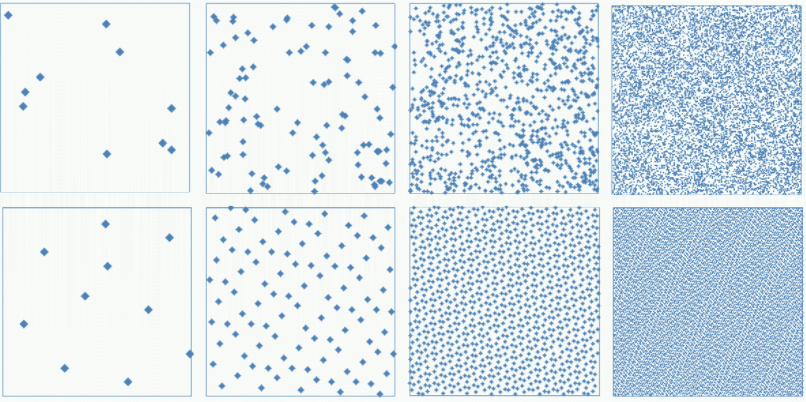
\includegraphics[width=0.7\linewidth]{graph/discrep}


Inconvénient : la suite $(X^{n+p}_0,...,X^{n+p}_{n+p-1})$ ne s'obtient pas en rallongeant la suite  $(X^n_0,...,X^n_{n-1})$. 



\subsection{Généralisation}



Le TCL  admet de nombreuses généralisations : En fait il suffit que les $X_n$ soient suffisamment décorrélées (au sens large) et que leur variance reste dans un intervalle borné pour que cela marche. 

On peut aussi voir ce théorème ainsi : En sommant un nombre important de v.a. suffisamment indépendantes, on est proche d'une gaussienne (pas forcément centrée-réduite). 



\subsection{Intervalle de confiance}

Plaçons nous dans la situation suivante : vous disposez de plusieurs appareils pour mesurer la température. Tous ces appareils font des erreurs aléatoires. On suppose que tous ces appareils sont indépendants et tous identiques (= de même loi).


Notons $X_{:n}=[X_0,...,X_{n-1}]$ ces mesures. Notons $\mu$ la vraie température. On suppose que nos appareils ne sont pas biaisés, donc $\mathbf E[X_i]=\mu$. On note $\sigma^2$ la variance des $X_i$.

 On  estime naturellement $\mu$ par $\mean(X_{:n})$. On aimerait construire un intervalle de confiance pour cette estimation, càd trouver une va $a>0$ telle que
$$
\Pr[   -a<\mu<a  ] =  1-\alpha
$$
avec $\al=5\%=0.05$ par exemple.  


Par le TCL on a que 
$$
\frac {\mu- \mathrm{mean}(X_{:n})}{\frac {\si}{\sqrt{n}}}   \sim \bo N(0,1)
$$
Notons $q_\al>0$  le réel tel que $\Pr[ -q_\al < \bo N(0,1) <+q_\al  ] = 1-\al$. On le calcule avec l'inverse de la fonction de répartition = la fonction quantile = probability percentile function = ppf :
$$
q_\al = \mathrm{ppf}(1 - \frac \al 2)
$$

\dessin

On a:
$$
\Pr\Big[  - q_\al <  \frac {\mu- \mathrm{mean}(X_{:n})}{\frac {\si}{\sqrt{n}}}   <  + q_\al   \Big]  = 1-\al
$$
Donc
$$
\Pr\Big[     \mathrm{mean} (X_{:n}) - \frac {\sigma q_\al }{\sqrt{n}} \  < \ \mu \  < \   \mathrm{mean} (X_{:n}) +  \frac {\sigma q_\al }{\sqrt{n}}   \Big]  = 1-\al
$$
On a trouvé l'intervalle qui va bien. Remarquons qu'il se resserre quand $n$ grandi.



\section{Vecteur aléatoires}

Par défaut, les vecteurs seront considérés comme des colonnes. En particulier, lorsque $a$ est une matrice et $b$ un vecteur de taille compatible, on peut définir le produit matriciel   $ab$ qui donne un vecteur colonne.    


\subsection{Vecteur aléatoire}

Considérons un vecteur aléatoire $X \in \mathbb R^p$.  

\begin{itemize}
\item L'espérance de $X$ c'est le vecteur $\mu = \mathbf E[X]$ défini par $\mu_i = \mathbf E[X_i]$. 
\item la matrice de covariance de $X$ c'est la matrice $\sigma^2=\mathbf V[X]$ définie par $\si_{ij}= \mathrm{cov}(X_i,X_j)$. On peut l'écrire avec une multiplication matricielle:
$$
\sigma^2 = \mathbf E[ (X-\mu)  (X-\mu)^T ] \eqno{(SigmaMat)}
$$ 
(où nous supposons, comme pour les vecteurs, que l'espérance d'une matrice aléatoire, c'est la matrice des espérances). 

\item La matrice $\sigma^2$ est symétrique et ses valeurs propres sont positives.   Donc on peut l'écrire 
$$
\sigma^2=U  S^2  U^T
$$
 avec $S^2$ la matrice diagonale formée des valeurs propres (=valeurs singulières) que l'on classe dans l'ordre décroissant $s_{0}^2>s_{1}^2 >... $,   et $U$  une matrice orthogonale  (=  les colonnes   forment une base orthonormale =  les lignes   forment une base orthonormale)
 \end{itemize}
 
 
\subsection{Interprétation géométrique de la covariance} 

Considérons un vecteur aléatoire $X$ de matrice de covariance $\sigma^2= U S^2 U^T$. Noons $U_{i}$ les colonnes de $U$.   On note naturellement $s_i$ les racines carrées des $s^2_i=S^2_{i,i}$.   Elles sont ordonnées  $s_0>s_1 >... $.   On note $\mu$ le vecteur espérance de $X$.    Si maintenant nous simulons des copies indépendantes de $X$, elles formeront un nuage de point autour de $\mu$, dont la dispersion sera décrite par  les $U_i$  et $s_i$ :  

\dessin
 
en particulier, quand un des $s_i$ s'annule, le nuage est écrasé :
 
 \dessin
 
 
 
 Attention 1 : même en classant les valeurs propres par ordre décroissant, il n'y a pas unicité de la base $U$ (il y a un choix à faire quand des valeurs propres sont égales). 
 
Attention 2 :   tous les vecteurs aléatoires ne se répartissent pas en patate. Voici des simulations de vecteurs aléatoires de $\mathbb R^2$ qui admettent tous la matrice identité pour matrice de covariance (merci wikipedia). 
 

 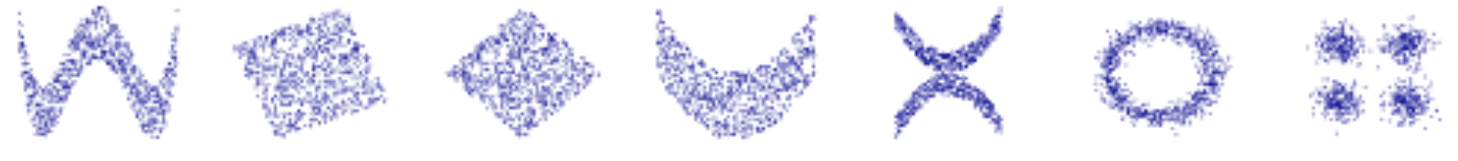
\includegraphics[width=\linewidth]{graph/identite}
 

 \subsection{Exo}
 
 \begin{exo}  \label{exoab}  Dans cet exo $a$ sera une matrice et $b$ un vecteur. Vérifiez ou complétez les points suivants: 
 \begin{itemize}
 \item $\mathbf E[aX+b] =a \mathbf E[X]+b$.
 \item $\mathbf V[aX+b] = a\mathbf V[X]a^T$. Aide: utilisez $(sigmaMat)$
 \item Soit $X$ un vecteur aléatoire de matrice de covariance  $\sigma^2=U S^2 U^T$ et d'espérance $\mu$.  Notons $\sigma = U S U^T$.  Quelles est la matrice de covariance de $\sigma^{-1} (X-\mu) $ ?  Faites le lien avec le fait de centrer-réduire les va. 
 \item $\sigma^2$ est symétrique et ses valeurs propres sont positives. La symétrie est évidente. Pour les valeurs propres, il suffit de montrer qu'elle est semi-définie positive. Vérifions-le : $\fo v :  v^T \sigma^2 v = ... \geq 0$. 
 \item Les coefficients de corrélation sont définis par  $c_{ij} =\mathrm{cov}(X_i,X_j)  / \sqrt{\mathbf V(X_i)} / \sqrt{\mathbf V(X_j)}  $.  Quelle fameuse inégalité permet d'affirmer que ces coefficients sont compris entre $-1$ et $+1$.
 \end{itemize}
  \end{exo}


\subsection{Dataframe}


Soit $(X^0,...,X^{p-1})$ un vecteur aléatoire (j'ai mis les indices en haut, car pour une fois, je le considère en ligne).  On en considère $n$ copies   $(X^0_i,...,X^{p-1}_i)_{i<n}$.   Notons \verb$X$ la matrice $\mathtt X_{ij} = X_i^j$.  Cette matrice s'appelle une dataframe.  

Dans une dataframe, les lignes  représentent  les individus et les colonnes leur caractéristique (age, sexe, taille, poids).   Les lignes sont indépendantes, mais pas les colonnes.  


Nous parlerons beaucoup de ces dataframe en analyse de données.  Pour l'instant nous nous contentons d'un exo.


\begin{exo} Considérons \verb$X$ une dataframe Que fait-on dans le programme python suivant :
\begin{verbatim}
X -=  np.mean(X,axis=0) 
X /=  np.std(X,axis=0,ddof=1) 
C  =  np.matmul(X.T,X)   
\end{verbatim}
Aide :  \verb$sum(X,axis=0) $ cela fait  $\sum_i X_{ij} $.  \verb$mean$ et  \verb$std$ fonctionnent de la même manière. 
\end{exo}






\subsection{Déformation de la densité}

Soit $X\in \mathbb R^p$ un vecteur aléatoire de densité $f$. Soit $a$ une matrice inversible $p\times p$. Soit $b\in \mathbb R^p$. Montrez que la densité de $aX+b$ est
$$
x\to   \frac 1 {|  \mathrm{det} \,a  |} f \Big(  a^{-1} (x-b)  \Big ) 
$$ 
Cela vous fera réviser votre formule de changement de variable.


\section{Vecteur gaussien}


Les vecteurs gaussiens sont les vecteurs aléatoires les plus naturels. 

On notera $I$ la matrice identité.  


\subsection{gaussien standart $\to$  gaussien général}


 \begin{definition}  Soit $Y\in \mathbb R^p$. On dit que $Y$ est un vecteur gaussien standart, et on note $Y\sim \bo N_p(0,I) $  lorsque les composantes $Y_i$  sont des $\bo N(0,1)$ indépendantes.  Son espérance est $0$ et sa matrice de covariance c'est $I$. 
\end{definition}

\begin{definition}
Les vecteurs gaussiens sont tous les vecteurs de la forme $a Y+b$ avec $a$ matrice, $b$ vecteur et $Y\sim\bo N_p(0,I)$. 
\end{definition}

 Ainsi par construction, la famille des vecteurs gaussiens est stable par combinaison affine. 



\subsection{ gaussien général $\to$ gaussien standart}

Ainsi, par définition, un vecteur gaussien général c'est $X= aY + b$ avec $Y \sim \bo N(0,I)$.  L'espérance de $X$ est alors $\mu = b$ et  sa matrice de covariance est alors $\sigma^2 = a a^T$ (cf. exo \ref{exoab}).  

Définissons alors $Y' := \sigma^{-1} (X-\mu)$ (attention, on ne retombe pas forcément sur $Y$).  On a que 
$$
X = \sigma Y' + \mu   \qq \mathrm{ et } \qq Y' \sim \bo N_p(0,I)
$$ 
Ci-dessus, on a une écriture "canonique" d'un vecteur Gaussien général (une écriture pas tout à fait unique car pour définir $\si$ il faut écrire $\sigma^2 = US^2 U^T$ et il peut y avoir des choix arbitraires  dans la construction de  $U$).   On voit bien avec cette écriture que la loi de $X$ ne dépend que de $\sigma^2$ et de $\mu$. On notera d'ailleurs:
$$
X \sim \bo N_p(\mu, \sigma^2)
$$ 



\subsection{Densité}

Si $Y\sim \bo N_p(0,I) $. Sa densité est le produit des densités des $Y_i$, c'est donc:
$$
f_Y(x)= \prod_i  \frac 1 {\sqrt{2\pi}}   e^{-\frac 1 2    x_i^2}  =  \frac 1 { (2\pi)^{\frac  n 2 }}   e^{-\frac 1 2  x^T  x }   
$$
Prenons maintenant $X \sim \bo N_p(0 ,\sigma^2)$. Puisque il peut s'écrire $\sigma Y$, sa densité est
$$
f_X(x) = \frac 1 { (2\pi)^{\frac  n 2 }   |\det \si|   }     e^{-\frac 1 2   (\sigma^{-1} x)^T   {\sigma^{-1} x} }     = \frac 1 { (2\pi)^{\frac  n 2 }   |\det \si|   }     e^{-\frac 1 2  x^{T}  \sigma^{-2}  {x} }   
$$

Remarque : on a utilisé implicitement que $\sigma^2$ étant inversible (= aucun des $s_i$ ne s'annule). Que se passe-t-il dans le cas contraire ? Et bien il n'y a pas de densité, ce qui est logique car : $\sigma^2$ non-inversible $\equi$  un des $s_i$ est nul $\equi$   $\si$ n'est pas de rang maximal  $\imp$    $X=\sigma Y$ est  porté par un sous-espace vectoriel strict de $\mathbb R^p$. 

Construisons un vecteur gaussien de dimension $2$ qui n'a pas de  densité:  Prenons $Y=[Y_0,Y_1] \sim \bo N_2(0,I)$.  Notons $X= [(Y_0+Y1)/2,(Y_0+Y1)/2  ]$. C'est un vecteur gaussien qui est porté par la diagonale. Comme la diagonale est d'aire nulle, $X$ n'a pas de densité.  
 
 

\begin{exo}
Ecrire la densité de $X\sim  \bo N_p(\mu,I)$ (placez $\mu$ au bon endroit)
\end{exo}





 \subsection{Covariance nulle et indépendance}

Rappelons que pour un vecteur $(X_0,X_1,...,X_{p-1})$ la factorisation de la densité 
$$
f(x_0,x_1,...,x_{p-1}) = f_0(x_0) f_1(x_1)...f_{p-1}(x_{p-1})
$$ 
équivaut à l'indépendance.   Dans le cas particulier des vecteurs gaussiens, on voit que la densité se factorise ssi $\sigma^2$ est diagonale. 

En fait ce résultat est vrai même quand le vecteur gaussien n'a pas de densité (= $\sigma^2$ non inversible). 


 \begin{exo} Un de vos camarades vous affirme que :  lorsque $X_1$ et $X_2$ sont deux va  gaussiennes alors
 $
 X_1\indep X_2 \equi  \mathrm{cov}(X_1,X_2) = 0
 $
Mais s'il écrit cela à l'interro, le prof ne sera pas content. Aidez-le à corriger son imprécision. 
  \end{exo}
 
 
 \subsection{TCL en dimension $p$}
 
Le TCL se généralise aux vecteurs aléatoire. Nous traitons ceci au via un exercice. 
 
 Considérons $K,L$ deux va indépendantes centrées réduites.  Définissons le vecteur $X=(X^0,X^1) = (K, K+L)$.  Prenons $(X_0,...,X_{n-1})$ des copies de $X$.   
 
 A quoi ressemble la loi de   $(X_0+X_1+...+X_{n-1})\in \mathbb R^2$  ? 
 
 Je ne vous demande pas de preuve, mais uniquement une intuition.  Vous pouvez aussi procéder par analogie avec le TCL en dimension 1. Vous pouvez aussi regarder sur internet, mais c'est la solution la moins marrante.  
 
 
 
 
 
 
 \section{Loi des estimateurs de l'espérance et de la variance}
  
 
 \subsection{Intro}
 
On dispose d'observation $X=[X_0,...,X_{p-1}]$. On calcule des estimateurs ex: $\mean(X), \std(X),...$. On aime bien ensuite connaitre la loi de ces estimateurs. Par exemple pour calculer des intervalles de confiance (cf. avant), ou bien pour faire des tests (cf. après).  Le calcul des lois exactes des estimateurs est souvent trop compliqué, sauf ...  quand  $X$ est un vecteur gaussien !  Et quand $X$ n'est pas gaussien, mais que $p$ est grand, les lois des estimateurs sont proches des lois qu'on obtient dans le cas gaussien (merci le TCL). 
 
 
Dans cette section, nous calculons la loi du couple  $\mean(X), \std(X)$ quand $X\sim \bo N_p(0,I)$.  La technique utilisée (projection de vecteur gaussien) est assez générique. Dans votre vie future, si vous rencontrez des estimateurs plus complexes (ex: coefficient de régression), le calcul de leur loi sera probablement basé sur cette technique de projection de vecteur gaussien. 
  
  
  
\subsection{Loi du Chi2}


On dit que $Y$ suit une loi du $\chi_2$ à $p$ degrés de liberté (=degree of freedom=df)  lorsque qu'il existe $X \sim \bo N_p(0,I)$ telle que
$$
Y = \|X\|^2= X_0^2 + ...+ X_{p-1}^2   
$$
On note $Y \sim \chi_2(df:p)$ ou plus simplement $\chi_2(p)$.   Comme d'habitude, si $k>0$ est une constante, on note $kY \sim \chi_2(df:p,scale:k)$.


Propriété : Quand $Y \sim \chi_2(p)$ on a 
 \begin{alignat}{1}
 \mathbf E[Y] &=  p \\
 \mathbf V[ Y] &= 2p 
 \end{alignat}




  
 
\subsection{Projection}

\begin{exo} 
Soit $Y \sim \bo N_p(0,I)$. Soit $U$ une matrice orthogonale. Montrez que   $UY \sim \bo N_p(0,I)$.  En d'autre terme: les lois $\bo N_p(0,I)$ sont invariante par rotation et symmétrie.  Aide : $UY$  est un vecteur ......   et  donc sa loi est caractérisée par ...... et .....  qui se calculent facilement. 
\end{exo}
 
 
 \begin{proposition}
 Soit $E$ un sous espace vectoriel de $\mathbb R^p$  et $E^\perp$ sont orthogonal.   Soit $Y \sim \bo N_p(0,I)$. Les projections $\Pi_E Y$ et $\Pi_{E^\perp} Y$ sont indépendantes. 
 \end{proposition}
 
 Démo : Considérons $U$ une matrice orthogonale, dont les premières colonnes $U_{:k}$ forment une base de $E$ et les dernières colonnes $U_{k:}$ forment une base de $E^\perp$.       Le vecteur $U^{-1} Y$ est l'expression de $Y$ dans la base $U$.  D'après l'exercice précédent,  $\tilde Y = U^{-1} Y$ suit une loi $\bo N_p(0,I)$, donc ses coordonnées sont  indépendantes. Ainsi: 
 $$
 \Pi_E Y = U   \tilde Y_{:k}    \qq  \indep  \qq \Pi_{E^\perp} Y  =  U   \tilde Y_{k:} 
 $$
 
 
 
 \subsection{Théorème de cochrane}
 
 Pour une échantillon $X=[X_0,X_1,...,X_{p-1}]$ quelconque, la loi de $\mean(X)$ et $\std^2(X)$ est impossible à calculer. Mais dans le cas gaussien : 
  
 
 \begin{theoreme} Considérons $X=[X_0,X_1,...,X_{p-1}]$ un échantillon de va de loi  $\bo N(\mu, \sigma ^2)$. En d'autres termes $X\sim \bo N_p(\mu \mathbf 1, \sigma^2 I )    $).      On a :
 \begin{itemize}
 \item  $\mean(X)$ et $\std^2(X)$ sont indépendants. 
 \item $\mean(X)$ suit une $\bo N(\mu ,\frac {\sigma^2} p)$. 
 \item $\frac{\std^2(X)} {\sigma^2}$ suit une loi $\chi_2(df: p-1,scale: \frac 1 {p-1})$. 
 \end{itemize}
 \end{theoreme}
 
 Exo : Du troisième point, on peut en déduire que $\std^2(X)$ est non biaisé (mais on avait déjà fait cet exo en dehors du cadre gaussien). 
 
 Exo : Sauriez-vous construire une région de confiance pour le couple $(\mu,\si)$, c'est à dire un ensemble  $A\subset \mathbb R^2$, dépendant de $X$, tel que $\Pr[(\mu,\si)\in A] = 0,95$ ?  
 
 Démonstration: Quitte à remplacer $X$ par $(X-\mu)/\sigma$, on peut supposer que $\mu=0$ et $\si=1$.  
 
 L'application $\mathbb R^p\to \mathbb R^p,  x\to \mean(x)$ est la projection  sur la diagonale de $\mathbb R^p$. Donc l'application $x\to x-\mean(x)$ est la projection  sur  l'orthogonale de la diagonale.    
  Donc  $\mean(X)$ est indépendant de $X-\mean(X)$.   Considérons une base orthonormale dont le premier vecteur est dans la diagonale.  Notons $\tilde X$    l'expression de $X$ dans cette base.  Ainsi $\mathrm{mean}(X) = \tilde X_0$ suit une loi $\bo N(0,1)$, tandis que $[\tilde X_{1}... \tilde X_{p-1}]  \sim \bo N_{p-1}(0,I)$. La norme euclidienne ne dépend pas du système de coordonnées (= de la base orthonormale choisie), ainsi  :  
$$
\| X-\mean(X)\|^2 = \| (\tilde X_1,...,\tilde X_{p-1})\|^2    \sim \chi_2(df:p-1)
$$
 \carre
 
 
 
 
 


\section{TCL sans connaitre la variance}


\subsection{Définition de la loi $t$ de Student.}



On dit que $Y$ suit une $t$ de Student à $p$-degré de liberté lorsqu'il existe deux va $Z,U$  indépendantes avec $Z \sim N(0,1)$  et $U \sim \chi_2(df=p)$   et que    
$$
Y= \frac Z  {\sqrt{\frac U p }} 
$$
On note alors $Y \sim t(df:p)$ ou plus simplement $Y \sim t(p)$




\subsection{Une sorte de TCL}


 
On considère un échantillon :  $X = [X_0,...,X_{p-1}]$  représentant des observations iid d'une quantité.

On note comme d'habitude $\mu$ et  $\sigma$ l'espérance et l'écart-type de $X_0$.  Ce sont des caractéristiques de la vraie quantité. Si on n'y a pas accès, on les estime par  $\mean(X) $ et $\std(X)$.    

Maintenant nous aimerions répondre à la question suivante :
        <<de combien  $\mean(X)$ et $\mu$ sont éloignés ? >>

Pour répondre avec le TCL, nous utilisions : 
$$
\frac{\mean(X) - \mu }{ \frac{\si}{\sqrt{p}}  }   \sim \bo N(0,1) 
$$
Mais en général, on ne connait pas $\sigma$, on le remplace par son estimateur. Définissons: 
$$
R(X) := \frac{\mean(X) - \mu }{ \frac{ \std(X) }{\sqrt{p}}  }  
$$
Quand $p$ est grand, $\si$ et $\std(X)$ sont très proches, et on peut affirmer que $R(X)\sim \bo N(0,1) $.  

Mais quand  $p$ est petit, le hasard peut donner des valeurs de $\std(X)$ très petites, donc des valeurs de $R(X)$ très grandes.  Du coup on s'attend à ce que la loi de $R(X)$  ait des queues plus lourdes que celle de la gaussienne.


La loi exacte de $R(X)$  est impossible à calculer dans le cas générale.
Mais on peut supposer que chaque observation $X_i$  est proche d'une gaussienne
(car chaque observation est sans doute elle-même la somme de plusieurs phénomènes indépendants). 

\begin{theorem} Quand $X_0,...,X_{p-1}$ sont iid de loi $\bo N(\mu,\sigma^2)$ on a : 
$$
\mathrm{loi} ( R(X) )   = t( p-1) 
$$
\end{theorem}


\subsection{Démo}

Première étape : On peut écrire $X = \sigma Y + \mu$  avec $Y \sim \bo N(0,1)$. Et en recalculant le rapport $R(X)$, on trouve :
$$
  R(X)= \frac{\mean(Y) }{ \frac{\std(Y)}{\sqrt n}  }
$$
Donc on peut supposer dès le début que $\mu=0$ et $\sigma^2=1$.    On suppose donc désormais que $X \sim \bo N_p(0,I)$. 


Seconde étape : à faire vous même en utilisant le théorème de Cochrane. 



\subsection{Conclusion}


A la réponse    <<de combien  mean(X) et $\mu$ sont éloignés ? >> on peut répondre dans le cas gaussien :
$$
    \mean(X) - \mu  \sim \frac{\std(X)}{\sqrt{p}}  \    t(p-1) 
$$
quand $p$ est grand, on retombe sur le TCL. Quand $p$ est petit, il faut se méfier des queues de la Student : la  "constante aléatoire" $t(p-1) $ peut-être très grande. 


La plupart du temps, quand on estime un paramètre par une moyenne d'observation, on a au moins 20 observations (en dessous de 20 observations, on est plus voyant que statisticien).  Or  dès $p=20$, $\si$ et $\std$ sont très proches.       Aurait-on fait tout ceci pour rien ?  Non, car  ce travail est juste un cas d'école. Dans la vraie vie, les estimateurs sont plus complexes et les degrés de liberté différents. Par exemple, quand on fait de la regression linéaire avec $p$ observations et $d$ variables explicatives, on tombe sur des estimateurs qui, une fois renormalisés, suivent des lois $t(p-d-1)$.     Attention aux queues lourdes quand $d$ est grand !



\section{Tests statistiques}


\subsection{Test avec statistique positive}

On a deux hypothèses:  $H_0$ et son contraire $H_1$.  Exemple 1: 

\begin{tabular}{ll}
$H_0:$ les hommes boivent autant de bière que de vin \\
$H_1:$ les hommes ne boivent pas autant de bière que de vin. 
\end{tabular}

Exemple 2:

\begin{tabular}{ll}
$H_0:$ l'échantillon observé est a une distribution gaussienne. \\
$H_1:$l'échantillon observé est n'a pas une distribution gaussienne. 
\end{tabular}


Exemple 3: 

\begin{tabular}{ll}
$H_0:$ Le sexe et le QI sont indépendants. \\
$H_1:$ Le sexe et QI ne sont pas indépendants. 
\end{tabular}




Notez que les deux hypothèses ne sont pas interchangeable : $H_0$ est une hypothèse "précise", et donc sont contraire $H_1$ est une hypothèse "vague". 


On construit une "statistique" $D>0$.  On a construit $D$ pour qu'en théorie :

\begin{tabular}{ll}
$H_0$  &$\imp$  $D$ petit. \\
$H_1$  &$\imp$  $D$ grand
\end{tabular}

Ainsi en pratique, on effectue des observations pour calculer $D$ et :

\begin{tabular}{ll}
$D \leq$ seuil  &$\imp$    on choisit $H_0$ \\
$D >$  seuil &$\imp$   on choisit $H_1$
\end{tabular}

Mais comment choisir le seuil ?  En fait, en construisant $D$ on a fait en sorte que :

\begin{tabular}{ll}
$H_0$  &$\imp$  $D$ suit une loi de fonction de répartition $F$ bien connue (ex :   $\chi_2$). \\
$H_1$  &$\imp$  $D$ est très très grand. 
\end{tabular}

En général, puisque $H_1$ est une hypothèse "vague",  sous $H_1$ on a beaucoup mal à évaluer la loi de $D$, on sait juste qu'il est grand.



Le principe de tous les tests est que : 
\begin{center}
<<Quand $H_0$ est vrai, on veut choisir $H_1$ rarement>>. 
\end{center}
On se fixe  un $\al$ petit (ex: $0.05$). C'est le niveau du test.  Et on souhaite que, sous $H_0$, la probabilité de choisir $H_1$ soit de $\alpha$.  Ainsi : Sous $H_0$ :
$$
\Pr[D>seuil] = \alpha  \equi  \Pr[D\leq seuil] = 1-\alpha \equi F(seuil) = 1-\alpha \equi  seuil = F^{-1} (1-\alpha)
$$
C'est la méthode la plus simple qu'on a trouvé pour dire précisément que  $D$ est grand ou petit. 


\begin{remarque} on aurait aussi pu choisir comme critère :
\begin{center}
 <<Quand $H_1$ est vrai, on veut choisir $H_0$ rarement>> 
\end{center}
mais c'est beaucoup plus dur car, sous $H_1$, on connait en général mal la loi de $D$.
\end{remarque}


Donc en résumée
\begin{tabular}{ll}
$D \leq  F^{-1}(1-\alpha)$   &$\imp$    on choisit $H_0$ \\
$D > F^{-1}(1-\alpha)$    &$\imp$   on choisit $H_1$
\end{tabular}


\subsection{$p$-valeur}

Mais l'histoire ne s'arête pas là, car on aimerait avoir un critère quantitatif pour dire si on choisit $H_1$ franchement, ou du bout des lèvres. On a :
$$
\{\mathrm{choisir } H_1\} \equi D > F^{-1}(1-\alpha) \equi F(D) >1- \alpha \equi 1 -F(D) \leq \alpha
$$
On définit alors $p$-valeur =  $1 -F(D)$ et du coup, plus cette $p$-valeur est petite est plus l'hypothèse $H_1$ est la bonne. 

\begin{tabular}{lll}
$p$-valeur & $\sim  0$    &$H_1$ est $\star\star\star$ \\
$p$-valeur & $\sim  0.01$    &$H_1$ est $\star\star$ \\
$p$-valeur & $\sim  0.05$    &$H_1$ est $\star$ \\
$p$-valeur & $\sim  0.1$    &$H_1$ est  bof 
\end{tabular}


\subsection{Exemple : le test du $\chi_2$ de Pearson}

On dispose de deux dès : un rouge et un noir.
On voudrait savoir si l'un des deux est truqué.
On les fait rouler 60 fois chacun. On trouve les effectifs suivants : 
\begin{alignat*}{1}
black &= [9, 10, 12, 11, 8, 10]\\
red &=  [6, 5, 14, 15, 11, 9]
\end{alignat*}
A l'oeil :  pensez-vous qu'un des deux dés est truqué ?

Que prendriez-vous pour:
  \begin{tabular}{ll}
$H_0$  &:   ... \\
$H_1$  & :  ...
\end{tabular}

      
 La statistique  de Pearson (= distance du $\chi_2$) est donnée par :

$$
D= \sum_i \frac{ (f_{obs}[i] - f_{exp}[i] ) )^2 }{ f_{exp}[i] }
$$
Avec :\\
$ f_{obs}[i]$  : effectif observé dans la classe $i$. \\
$f_{exp}[i]=10$ : effectif attendu dans la classe $i$

Notons $J=6$ le nombre de classes possibles. On a :

\begin{tabular}{ll}
$H_0$  &$\imp$  $D\sim  \chi_2 (J-1)$.  \\
$H_1$  &$\imp$  $D \sim + \infty $. 
\end{tabular}

Attention : si on veut être précis : sous $H_0$ on a une convergence en loi vers $ \chi_2 (J-1)$ (quand le nombre de lancés tend vers l'infini), tandis que sous $H_1$ on a une convergence p.s. vers $\infty$ ; ça c'est facile à voir avec la loi forte des grands nombres.



\subsection{Le test du $\chi_2$ de Pearson (suite)}


Le test de Pearson juge de l'adéquation entre une série de données (=observed) et une loi de probabilité définie a priori (=attendue=expected).

La loi à priori peut-être discrète (ex: Poisson) ou continue (ex: Normale).

Dans les deux cas, on se ramène à $J$ classes  en découpant le support de la loi attendue. Ex :
\begin{itemize}
\item Poisson, on peut prendre $[0], [1], [2,3], [4,5,6], [7,..., \infty[ $  donc $J=5$
\item Normale, on peut prendre  $]-\infty,-1], [-1,1], [1,+\infty[$             donc $J=3$
\end{itemize}
Ces classes doivent être assez nombreuses pour ne pas perdre trop d'information mais, à l'inverse,
doivent contenir un minimum de valeur de la distribution attendue.
En général, on fait en sorte qu'il y ai 5 observations par classe.

Si la loi de probabilité théorique dépend de paramètres (moyenne, variance...) inconnus au moment du test,
les données peuvent être utilisées pour estimer ceux-ci, ce qui facilite l'adéquation.
Il faut alors diminuer le nombre de degrés de liberté du nombre de paramètres estimés. 

En l'absence d'estimation,  le nombre de degré de liberté est de $J-1$


Nous verrons en TP comment ce test général peut-être utiliser pour tester l'indépendance d'un couple de va. 



\subsection{Test avec une statistique signée}

C'est une très légère variante du test avec une statistique positive. On écrit  quand même les détails, car c'est dans les détails que se cachent les erreurs.  


On a deux hypothèses:  $H_0$ et sont
 contraire $H_1$.  
On construit une "statistique" $T$ pour qu'en théorie :

\begin{tabular}{ll}
$H_0$  &$\imp$  $|T|$ petit. \\
$H_1$  &$\imp$  $|T|$ grand
\end{tabular}

Ainsi en pratique, on effectue des observations pour calculer $T$ et :

\begin{tabular}{ll}
$|T| \leq$ seuil  &$\imp$    on choisit $H_0$ \\
$|T| >$  seuil &$\imp$   on choisit $H_1$
\end{tabular}

Mais comment choisir le seuil ?  En fait, en construisant $T$ on a fait en sorte que :

\begin{tabular}{ll}
$H_0$  &$\imp$  $T$ suit une loi de fonction de répartition $F$  (ex :  gaussienne ou student). \\
$H_1$  &$\imp$  $T$ est très  grand en valeur absolue. 
\end{tabular}


Le principe de tous les tests est que : 
\begin{center}
<<Quand $H_0$ est vraie, on veut choisir $H_1$ rarement>>. 
\end{center}
On se fixe  un $\al$ petit (ex: $0.05$). C'est le niveau du test.  Et on souhaite que, sous $H_0$, la probabilité de choisir $H_1$ soit de $\alpha$.  Ainsi : Sous $H_0$ :
$$
\Pr[|T|>seuil] = \alpha  \equi  \Pr[|T| \leq seuil] =1- \alpha \equi    \Pr[-seuil \leq T \leq seuil]  =1- \alpha   \equi  seuil = F^{-1} (1-\frac {\alpha}2)
$$


Donc en résumé

\begin{tabular}{ll}
$|T| \leq  F^{-1}(1-\frac {\alpha}2)$   &$\imp$    on choisit $H_0$ \\
$|T| > F^{-1}(1-\frac {\alpha}2)  $     &$\imp$   on choisit $H_1$
\end{tabular}


On aimerait avoir un critère quantitatif pour dire si on choisit $H_1$ franchement, ou du bout des lèvres. On a :
$$
\{\mathrm{choisir } H_1\} \equi      |T| >  F^{-1}(1-\frac {\alpha}2)        \equi F(|T|) >    (1-\frac {\alpha}2) \equi 1 -F(|T|) \leq \frac {\alpha}2 \equi 2 [1 -F(|T|)] \leq \alpha 
$$
On définit alors $p$-valeur =  $2 [1 -F(|T|)]$ et du coup, plus cette $p$-valeur est petite et plus l'hypothèse $H_1$ est la bonne. 



Il faut absolument que vous soyez capable de refaire cette série de calcul sur une feuille, sans regarder aucune note. Beaucoup d'erreur (ex: dans les blog) proviennent 
 d'une confusion entre $\al, 1-\al$ ou entre $\al $ et $\frac \al 2$ ou entre une loi du $\chi_2$ et une loi de Student.   



\subsection{Exemple : le test de Student}

\begin{tabular}{ll}
$H_0:$ les hommes boivent autant de bière que de vin \\
$H_1:$ les hommes ne boivent pas autant de bière que de vin. 
\end{tabular}

On considère  $p$ individu. On note $X_i$  la différence entre les verres de bière et les verres de vin consommés par l'individu $i$.  On note $\mu=\mathbf E[X_0]$.   Ainsi 
\begin{tabular}{ll}
$H_0:$  $\mu=0$ \\
$H_1:$  $\mu \neq 0$. 
\end{tabular}

On définit la statistique
$$
T = \frac {\mean(X) }{ \frac {\std(X)} {\sqrt{p}}   }  \eqno{(def T)}
$$


Sous $H_0$, $\mu=0$, et  $T=R(X)$ dont nous avions calculé la loi : c'est une $t(p-1)$. 

Sous $H_1$, $\mu\neq 0$, $\mean(X) \to \mu$, $\std(X) \to \sigma$, $\sqrt{p}\to \infty$ , donc $T$ tend vers $\pm \infty$ en fonction du signe de $\mu$. 



En TP nous verrons aussi une variante de ce test, quand on dispose de deux échantillons indépendants, dont on veut comparer les espérances. 


\subsection{vraie vie et grosse-donnée}


Un gros problème des tests : ils dépendent toujours de la taille de l'échantillon.

Typiquement, si on travaille avec des échantillons de taille 1 million issus de la 'vraie vie' (=non-simulés), les tests rejetteront toujours $H_0$ :
En effet, rappelons que $H_0$ est une hypothèse 'précise' qui suppose une égalité entre deux lois (ou deux espérances). 
 Or dans la 'vraie vie' il n'y a jamais d'égalité parfaite. Et  1 million de données permettent de détecter la plus infime différence.

 Cette triste vérité n'est pas assez connue.  En TP on l'appellera :  l'effet <<vraie vie et grosse-donnée>>

 A l'inverse, quand on a très peu de données, les tests ont tendance à beaucoup accepter H0 : c'est l'effet <<petite-donnée>>.


























\end{document}



 
  et toutes deux sont des Gaussiennes standart sur $E$ et $E^\perp$. 
 

\demo Considérons le vecteur 
$$X  =  \begin{pmatrix}
\Pi_{E} Y \\
\Pi_{E^\perp} Y
\end{pmatrix} 
 = 
 \begin{pmatrix}
\Pi_{E}  \\
\Pi_{E^\perp} 
\end{pmatrix} 
Y
 $$
  C'est un vecteur  gaussien dont la matrice-variance-covariance faut
  $$
  \mathbf V[X]  =  \begin{pmatrix}
\Pi_{E}  \\
\Pi_{E^\perp} 
\end{pmatrix}  
\mathbf V[Y]
( \Pi_{E} \Pi_{E^\perp}  )  =  
\begin{pmatrix}
\Pi_{E} & 0 \\
0 & \Pi_{E^\perp}
\end{pmatrix}
  $$
 Ainsi les deux parties de $X$ sont indépendantes. Déterminons la loi de ces parties. Par exemple la loi de $\Pi_E Y$. Puisque c'est un vecteur gaussien centré, il suffit de caculer sa matrice-covariance : 
 $$
 \mathbf V[\Pi_E Y] = \Pi^
 $$
 
 
  deux matrices de projections orthogonnes, alors
 
 $$
 \mathbf E[\ph(MY) \Psi(NY)] = \cst \int  \ph
 $$
 
 
 
